\documentclass[a4paper]{article}

\usepackage{graphicx}
\usepackage{caption}
\usepackage{listings}
\usepackage{color}

\definecolor{mygreen}{rgb}{0,0.6,0}
\definecolor{mygray}{rgb}{0.5,0.5,0.5}
\definecolor{mymauve}{rgb}{0.58,0,0.82}

\lstset{ %
  backgroundcolor=\color{white},
  basicstyle=\footnotesize,
  breakatwhitespace=false,
  captionpos=b,
  commentstyle=\color{mygreen},
  frame=single,
  keepspaces=true,
  keywordstyle=\color{blue},
  language=C,
  rulecolor=\color{black},
  stringstyle=\color{mymauve},
  tabsize=2,
  title=\lstname
}

\begin{document}

\title{
Development of Real-Time Systems\\
Assignment 4
}
\author{Elyasin Shaladi}
\maketitle

\tableofcontents
\newpage
\listoftables
\lstlistoflistings
\listoffigures

\newpage

\section{Simulation assignment}
The assignment is to use a real-time simulator to verify feasibility of a set of tasks.

\subsection{Simulation 1 --- EDF Scheduler}

Consider the tasks $T1(3, 0.5), T2(4, 1.5, 3), T3(7, 1.0, 5)$ and the EDF scheduler. A sporadic job arrives at $t=50$ having the execution time of $10$ and a relative deadline of $30$.

\begin{table}[!htbp]
\begin{center}
\begin{tabular}{|l||l|l|l|l|}
\hline
Task   & $p_i$ & $e_i$ & $D_i$ & $r_i$\\
\hline
\hline
Task 1 & 3 & 0.5 & 3 & 0\\
\hline
Task 2 & 4 & 1.5 & 3 & 0\\
\hline
Task 3 & 7 & 1 & 5 & 0\\
\hline
Task 4 & - & 10 & 30 & 50 \\
\hline
\end{tabular}
\caption{Task 1, 2 and 3 correspond to T1, T2 and T3. Task 4 is the sporadic task.}
\end{center}
\end{table}

\subsubsection{What is the minimum/maximum/average response time of all tasks?}

\begin{table}[!htbp]
\begin{center}
\begin{tabular}{|l||l|l|l|}
\hline
Task   & $min$ & $avg$ & $max$ \\
\hline
\hline
Task 1 & 0.5 & 0.676 & 1.5 \\
\hline
Task 2 & 1.5 & 1.7 & 2 \\
\hline
Task 3 & 1 & 1.967 & 3.5 \\
\hline
Task 4 & 29 & 29 & 29 \\
\hline
\end{tabular}
\caption{Response time statistics for EDF simulation.}
\end{center}
\end{table}

\subsubsection{Is any task missing the deadline? Which task? Where?}
All the tasks meet their deadlines.

\subsubsection{Is the sporadic job meeting its deadline?}
Yes, the sporadic job meets its deadline. It is released and executed at time $50ms$ and completes at time $79ms$.

\subsubsection{What is the response time for the sporadic job?}
The response time for the sporadic job is $29ms$.

\newpage

\subsection{Simulation 2 --- RM Scheduler}

Consider the tasks $T1(3, 0.5), T2(4, 1.5, 3), T3(7, 1.0, 5)$ and the RM scheduler. A sporadic job arrives at t=50 having the execution time of $10$ and a relative deadline of $30$.

\begin{table}[!htbp]
\begin{center}
\begin{tabular}{|l||l|l|l|l|}
\hline
Task   & $p_i$ & $e_i$ & $D_i$ & $r_i$\\
\hline
\hline
Task 1 & 3 & 0.5 & 3 & 0\\
\hline
Task 2 & 4 & 1.5 & 3 & 0\\
\hline
Task 3 & 7 & 1 & 5 & 0\\
\hline
Task 4 & - & 10 & 30 & 50 \\
\hline
\end{tabular}
\caption{Task 1, 2 and 3 correspond to T1, T2 and T3. Task 4 is the sporadic task.}
\end{center}
\end{table}

\subsubsection{What is the minimum/maximum/average response time of all tasks?}

The table shows that the sporadic job (Task 1) does not have response time statistics. The sporadic job should be rejected because it cannot meet its deadline.

\begin{table}[!htbp]
\begin{center}
\begin{tabular}{|l||l|l|l|}
\hline
Task   & $min$ & $avg$ & $max$ \\
\hline
\hline
Task 1 & 0.5 & 0.5 & 0.5 \\
\hline
Task 2 & 1.5 & 1.84 & 2 \\
\hline
Task 3 & 1 & 1.9 & 3 \\
\hline
Task 4 & - & - & - \\
\hline
\end{tabular}
\caption{Response time statistics for RM simulation}
\end{center}
\end{table}

\subsubsection{Is any task missing the deadline? Which task? Where?}
The sporadic task job Task 1 misses its deadline. In the simulation it starts at $t=50ms$ and is aborted at $t=80$ because it can not complete.

\subsubsection{Is the sporadic job meeting its deadline?}
No, the sporadic job does not meet its deadline.

\subsubsection{What is the response time for the sporadic job?}
The sporadic job is aborted at $t=80$ in the simulation. The sporadic job therefore would be rejected by the real-time scheduler and is not executed.

\subsubsection{Which scheduler is better in this example; EDF or RM?}
The EDF scheduler is better because with the same task set and the same sporadic task requirements EDF is schedulable, but RM is not schedulable.

\newpage

\section{Programming assignment}

In this programming assignment, we will handle aperiodic jobs in FreeRTOS. \\
I created the matrix task with the functionality given in the Assignment 2, which is a computationally intensive task. \\
\\
I also added a software timer to the \textit{main} function that triggers a software interrupt every $5$ seconds and added the timer callback function.  The timer is started just before the scheduler is started. \\

\begin{lstlisting}[label=Software timer,caption=Definition and start of the software timer]
	...
	/* Timer task */
	TimerHandle_t timer_handle = 0;
	timer_handle = xTimerCreate(
    	"Timer",					//Naming the timer
        5000 / portTICK_PERIOD_MS,	// The period of the timer: 5s
        pdTRUE,					//Make the timer expire periodically
        (void *) 0,			//Timer identifier (can be ignored)
        vTimerCallback	//Timer callback function
	);
    ...
	xTimerStart(timer_handle, 0);	//Start the timer
	vTaskStartScheduler();				//Start the real-time scheduler
    ...
\end{lstlisting}

The timer callback function creates an aperiodic task, which simulates a (dummy) workload. When the aperiodic task completes it is removed from the schedule. \\

\subsection{Is the system fast enough to handle all aperiodic tasks? Why?}

No, the system is not able to handle the aperiodic jobs because the aperiodic jobs are not assigned enough computing time due to their lower priority. The aperiodic tasks are created with priority $2$ while the matrix task has priority $3$. \\
You can see in the output below that the aperiodic tasks are started by the timer callback, but they do not complete before the next timer interrupt is triggered (i.e. they do not complete before the release/start of the next aperiodic task job). \\

\newpage

\begin{lstlisting}[label=Aperiodic job not completing,caption=The aperiodic job is started but does not complete in time]
  Matrix calculation done.
  Matrix calculation done.
  Matrix calculation done.
  Timer callback!
  Matrix calculation done.
  Aperiodic task started!
  Matrix calculation done.
  Matrix calculation done.
  Matrix calculation done.
  Timer callback!
  Matrix calculation done.
  Aperiodic task started!
  Matrix calculation done.
  Matrix calculation done.
  ...
\end{lstlisting}

\subsection{If not, solve this problem without alter the functionality of any task}

In order to solve this problem we can use the technique of Assignment 2. We define a priority task that verifies the state of the aperiodic job regularly and raises its priority to $4$ in order to allow it to execute. The aperiodc job will be able to complete before the next timer interrupt is triggered. \\
In order for this to work we have to set \textit{INCLUDE\_eTaskGetState} to $1$.\\

\begin{lstlisting}[label=Priority task,caption=Definition of the priority task]
/* Define the priority task function */
static void priority_task() {
	while (1) {
		if (eTaskGetState(&aperiodic_handle) == eReady)
			vTaskPrioritySet(aperiodic_handle, 4);
		vTaskDelay(1 / portTICK_PERIOD_MS);
	}
}
\end{lstlisting}

A real-time simulation shows that the aperiodic jobs complete in time.\\

\begin{lstlisting}[label=Aperiodic job completing,caption=The aperiodic job completes in time]
Matrix calculation done.
Matrix calculation done.
Matrix calculation done.
Timer callback!
Aperiodic task started!
Aperiodic task done!
Matrix calculation done.
Matrix calculation done.
Matrix calculation done.
Timer callback!
Aperiodic task started!
Aperiodic task done!
Matrix calculation done.
Matrix calculation done.
...
\end{lstlisting}

\subsection{What is the response time of the aperiodic task?}

In this project the tick rate corresponds to $1ms$. We can run the aperiodic task with a slight modification to measure the response time. In order for this to work we have to configure FreeRTOS and set the \textit{configUSE\_TICK\_HOOK} to $1$ and use the \textit{vApplicationTickHook} function to increment the tick count at each tick. \\
We then use the tick counts at the start and the end of the aperiodic task to calculate the response time of the aperiodic task.\\

\begin{lstlisting}[label=Aperiodic task response time,caption=Calculating response time of aperiodic task]
/* Define the aperiodic task function */
static void aperiodic_task() {
	double start_time = tickcnt;
	printf("Aperiodic task started!\n");
	fflush(stdout);
	long i;
	for (i = 0; i < 1000000000; i++)
		; //Dummy workload
	printf("Aperiodic task done! (Response time = %fs)\n",
			(tickcnt - start_time)/1000./ portTICK_PERIOD_MS);
	fflush(stdout);
	vTaskDelete(aperiodic_handle);
}
\end{lstlisting}

Below you can see an example of the execution FreeRTOS project displaying the response time of the aperiodic jobs.\\
You can see that the response time of the aperiodic task is roughly between $1.2$ and $1.4$ seconds. \\

\begin{lstlisting}[label=Response times of aperiodic tasks,caption=Response time of aperiodic tasks]
Matrix calculation done.
Matrix calculation done.
Matrix calculation done.
Timer callback!
Aperiodic task started!
Aperiodic task done! (Response time = 1.300000s)
Matrix calculation done.
Matrix calculation done.
Matrix calculation done.
Timer callback!
Aperiodic task started!
Aperiodic task done! (Response time = 1.220000s)
Matrix calculation done.
Matrix calculation done.
Matrix calculation done.
Timer callback!
Aperiodic task started!
Aperiodic task done! (Response time = 1.281000s)
Matrix calculation done.
Matrix calculation done.
Timer callback!
Aperiodic task started!
Aperiodic task done! (Response time = 1.346000s)
Matrix calculation done.
...
\end{lstlisting}

\subsection{Provide a screen-shot of the running system}

I use Eclipse for development. The screen-shot shows the project in execution.\\

\begin{figure}[!ht]
\begin{center}
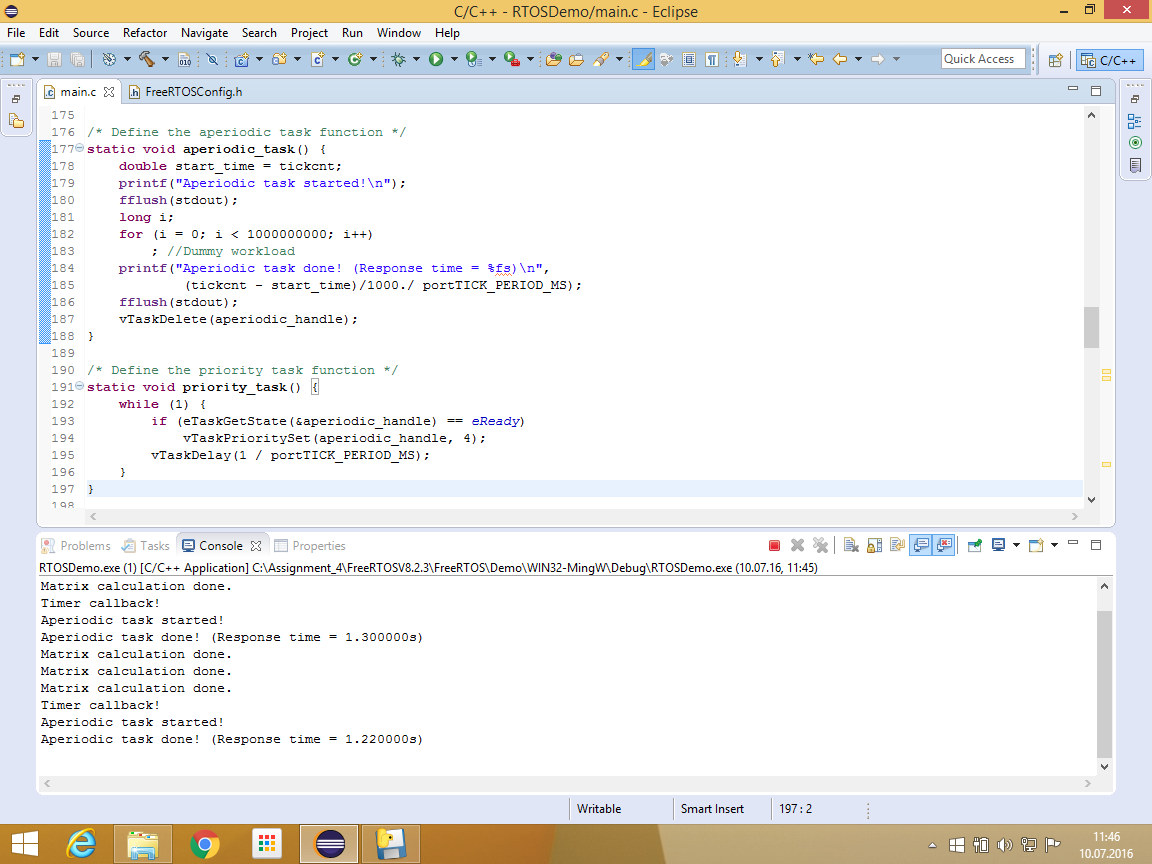
\includegraphics[width=\textwidth]{Assignment_4.png}
\caption{Screen-shot FreeRTOS scheduler execution}
\end{center}
\end{figure}

\end{document}
